\chapter{Architecture Constraints}

\section{Environment}
\label{sec:Environment}
In the context of an AUTOSAR ECU, RTA-SUM modules are technically built as Application Software Components. Therefore, each RTA-SUM module requires a full AUTOSAR SW stack to run. We assume that the following AUTOSAR SW will be used:
\input{generated/tables/tools.tex}

\section{Layers Definition}
The SUM\_TCS is a software module in the application layer of the standardized architecture of AUTOSAR (Figure~\ref{fig:Layers}). 
It interacts with other RTA-SUM modules and components of the BSW. In the latter case, the RTE is the means through which the interaction takes place.
\begin{figure}[htp]
\centering
	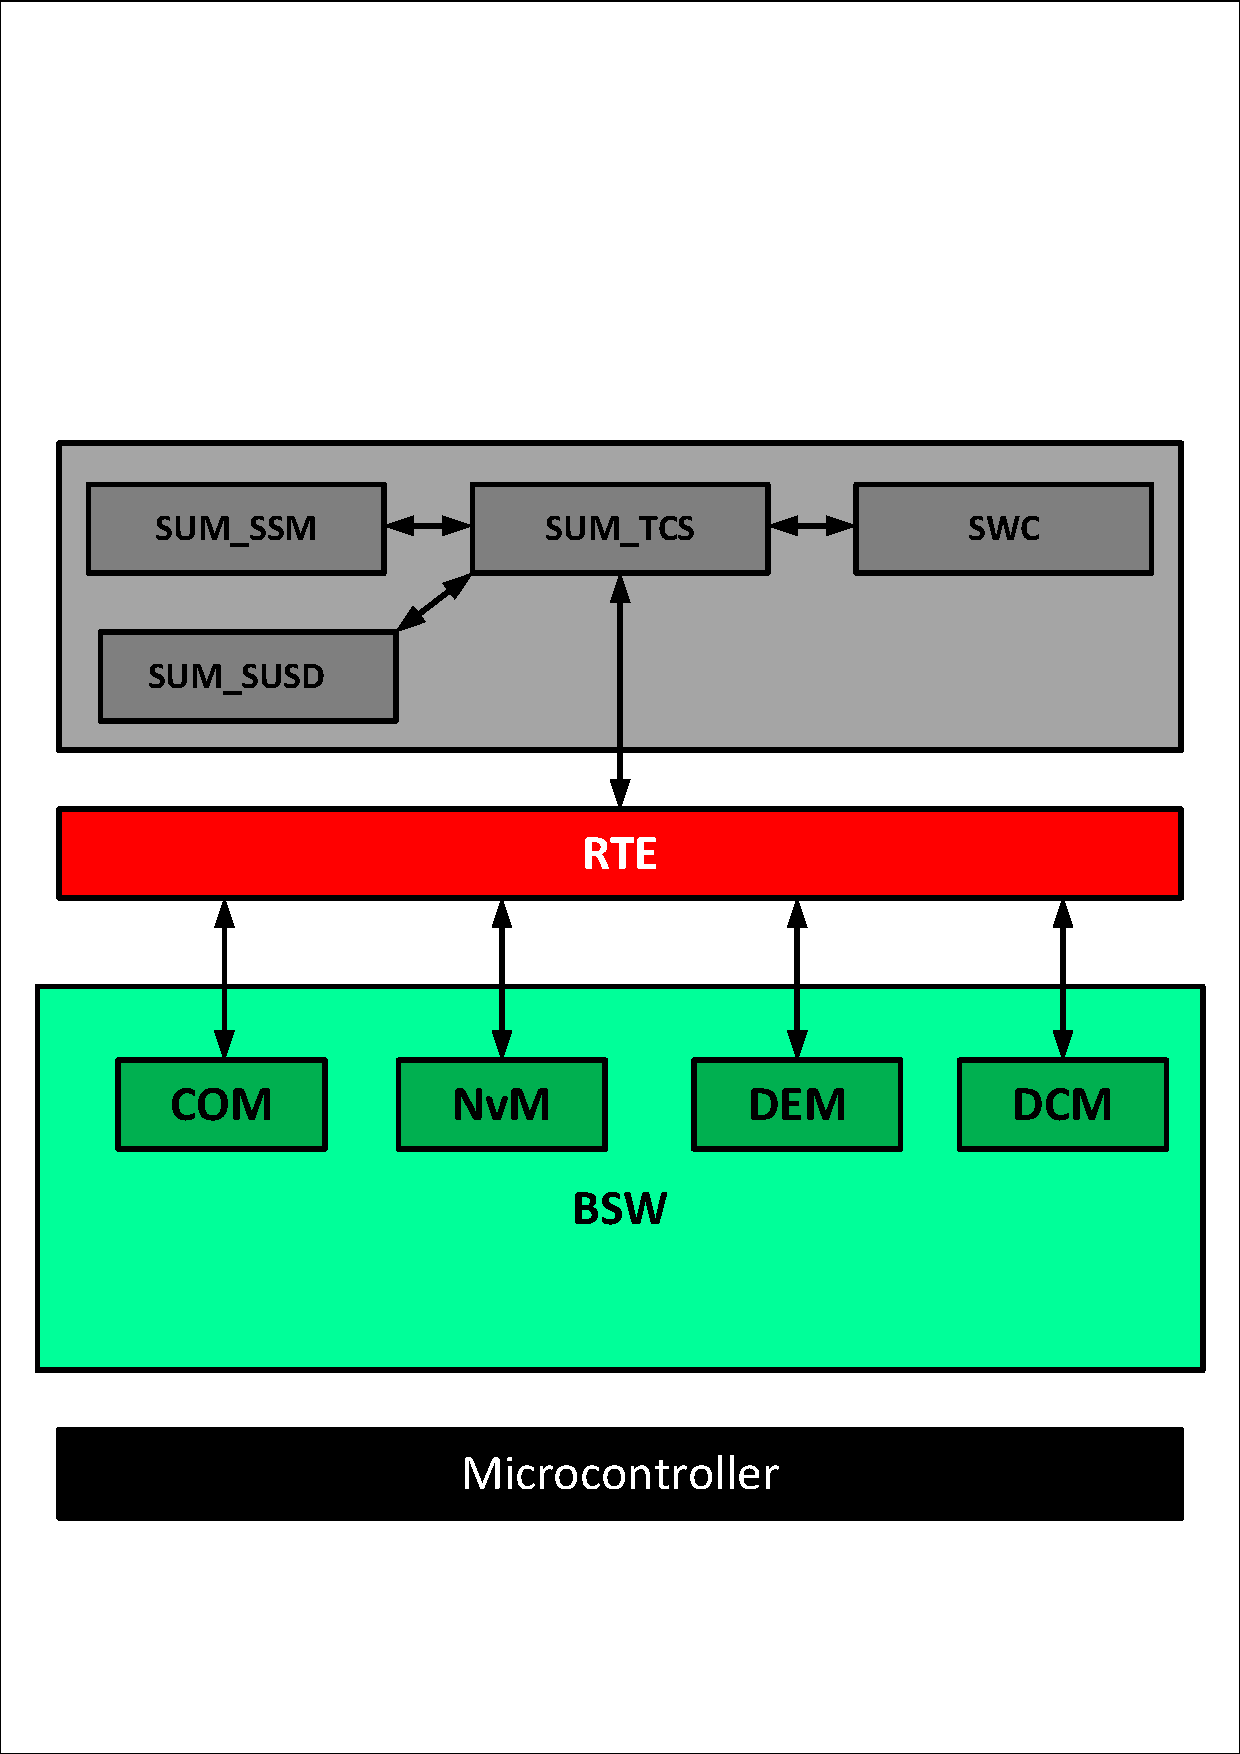
\includegraphics[scale=0.6]{images/Layers}
	\caption{System layer overview.}
	\label{fig:Layers}
\end{figure}

\section{Generic component interface}

The external interfaces of RTA-SUM module, and most of the interactions among SUM modules are specified in GM SDV-8002.

\section{Other constraints and assumptions}
At the scope of Timing Client Services (TCS), ECUs can be divided in TCS \textit{Master} or \textit{Slave}. 
The SUM\_TCS shall be implemented in ECUs that plays as TCS Slave, in which it shall be the unique TCS coordinator.
The usage of SUM\_TCS is reccomended for ECUs that set DTCs on public serial communication buses.
\\
\\
The usage of Time Synchronized output from SUM\_TCS is out-of-scope for this document.

%The SUM\_TCS shall be initialized after NvM Services being available in BSW.